\documentclass[tikz,border=8pt]{standalone}
\usepackage{amsmath,amssymb}
\usetikzlibrary{arrows.meta,calc,decorations.markings,decorations.pathmorphing,patterns,shapes.geometric,positioning}

\begin{document}
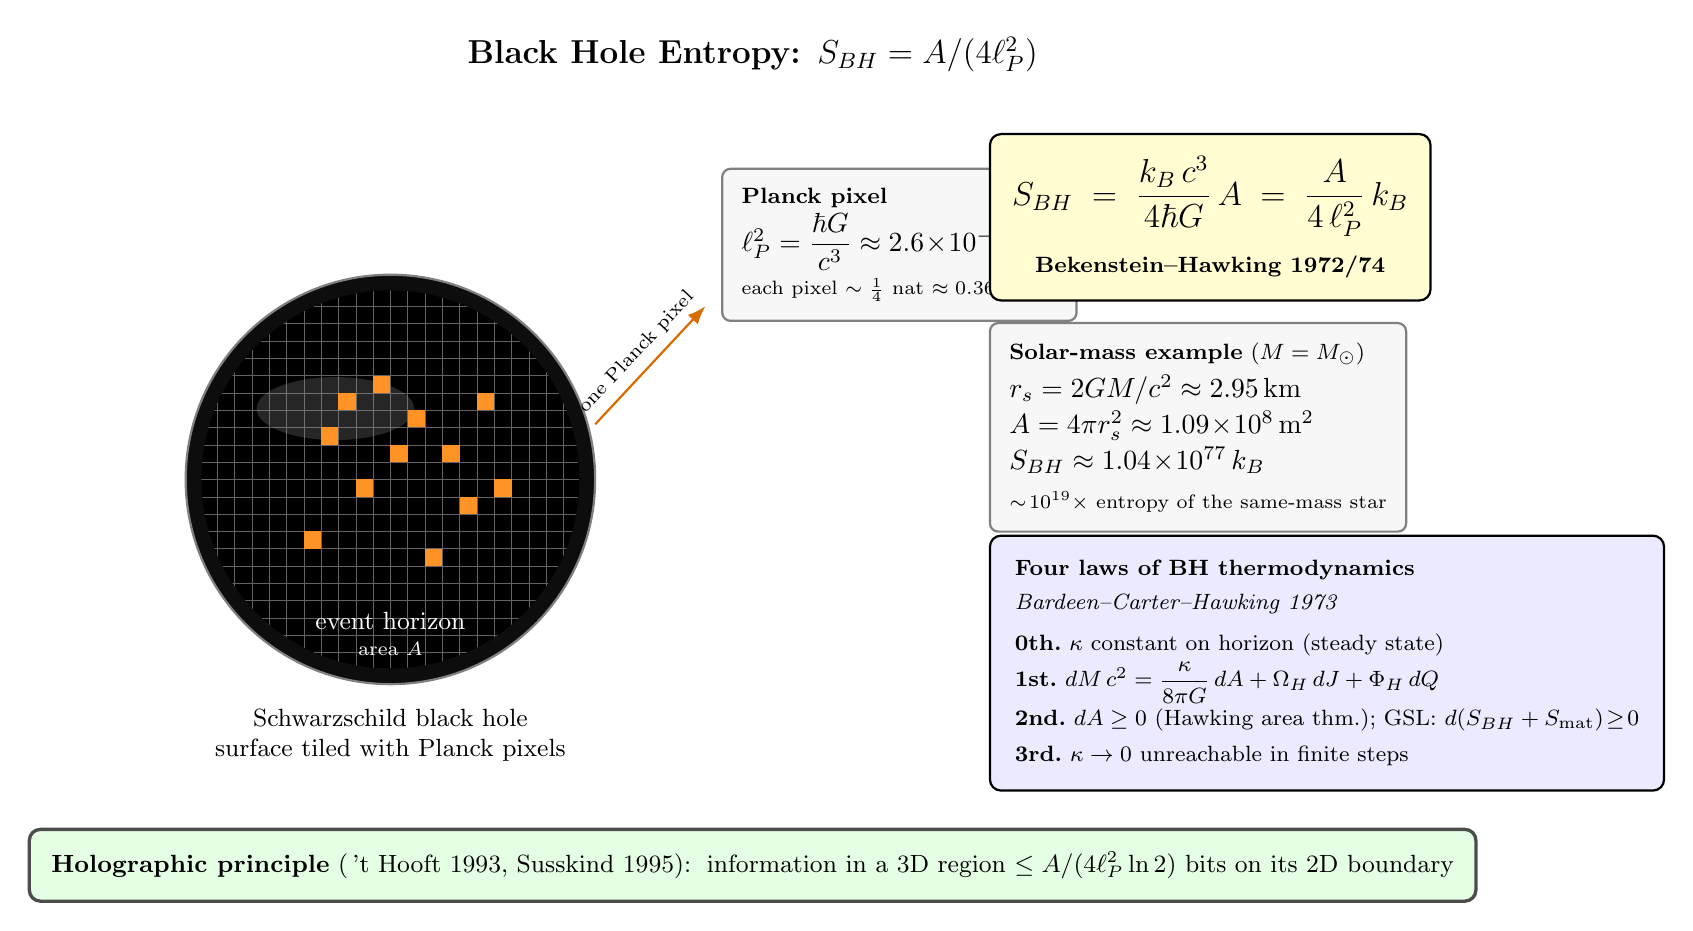
\begin{tikzpicture}[>=Latex,
  formulabox/.style={rectangle, draw=black, thick, rounded corners=4pt,
                     fill=yellow!18, inner sep=8pt, align=center},
  lawsbox/.style={rectangle, draw=black, thick, rounded corners=4pt,
                  fill=blue!8, inner sep=9pt, align=left},
  notebox/.style={rectangle, draw=black!50, thick, rounded corners=3pt,
                  fill=gray!6, inner sep=7pt, align=left}]

  % --- Title at top --------------------------------------------------------
  \node[font=\large\bfseries, align=center] at (0, 7.7) {%
    Black Hole Entropy: $S_{BH} = A/(4\ell_P^2)$};

  % ============================================================
  %  LEFT: black hole sphere with Planck-area pixel grid
  % ============================================================
  % Outer sphere shadow / event horizon disk
  \begin{scope}[shift={(-4.6, 2.3)}]
    % Filled black hole disk
    \fill[black!95] (0,0) circle (2.6cm);
    % Subtle gray rim
    \draw[black!50, thick] (0,0) circle (2.6cm);
    % Inner darker fill
    \fill[black!100] (0,0) circle (2.4cm);
    % Highlight to suggest 3D
    \fill[black!75, opacity=0.6] (-0.7,0.9) ellipse (1.0cm and 0.4cm);

    % Planck-area grid on the visible "front face" (light gray squares)
    % Use a clipped grid inside a circle to suggest tiling on the surface
    \begin{scope}
      \clip (0,0) circle (2.4cm);
      \draw[white!60!black, line width=0.18pt, opacity=0.65]
        (-2.4,-2.4) grid[step=0.22cm] (2.4,2.4);
    \end{scope}

    % Highlight a few "lit" pixels to emphasize each = 1 bit
    \foreach \x/\y in {0.22/0.66, 0.66/0.22, -0.44/-0.22, 0.88/-0.44,
                       -0.22/1.10, -0.88/0.44, 1.10/0.88, -1.10/-0.88,
                       1.32/-0.22, -0.66/0.88, 0.44/-1.10, 0/0.22}
      \fill[orange!85] (\x,\y) rectangle ++(0.22, 0.22);

    % Label horizon
    \node[font=\small, white] at (0, -1.8) {event horizon};
    \node[font=\scriptsize, white] at (0, -2.15) {area $A$};

    % Caption below
    \node[font=\small, align=center] at (0, -3.25) {%
      Schwarzschild black hole\\
      surface tiled with Planck pixels};
  \end{scope}

  % Arrow from a pixel to the side annotation
  \draw[->, thick, orange!85!black]
    (-2.0, 3.0) -- (-0.6, 4.5)
    node[midway, above, font=\scriptsize, sloped, black]
      {one Planck pixel};

  % Side annotation: Planck area
  \node[notebox, anchor=south west] at (-0.4, 4.3) {%
    \footnotesize\textbf{Planck pixel}\\[1pt]
    $\ell_P^2 = \dfrac{\hbar G}{c^3} \approx 2.6\!\times\!10^{-70}\,\mathrm{m}^2$\\[2pt]
    \scriptsize each pixel $\sim \tfrac{1}{4}$ nat $\approx 0.36$ bit};

  % ============================================================
  %  RIGHT TOP: main formula box
  % ============================================================
  \node[formulabox, anchor=north west] (formula) at (3.0, 6.7) {%
    \large $\displaystyle S_{BH} \;=\; \frac{k_B\,c^3}{4\hbar G}\,A
                            \;=\; \frac{A}{4\,\ell_P^2}\,k_B$ \\[6pt]
    \footnotesize\textbf{Bekenstein--Hawking 1972/74}};

  % Numeric example just below the formula box
  \node[notebox, anchor=north west] (example) at (3.0, 4.3) {%
    \footnotesize\textbf{Solar-mass example} ($M = M_\odot$)\\[2pt]
    $r_s = 2GM/c^2 \approx 2.95\,\mathrm{km}$\\[1pt]
    $A = 4\pi r_s^2 \approx 1.09\!\times\!10^{8}\,\mathrm{m}^2$\\[1pt]
    $S_{BH} \approx 1.04\!\times\!10^{77}\,k_B$\\[2pt]
    \scriptsize $\sim\!10^{19}\times$ entropy of the same-mass star};

  % ============================================================
  %  RIGHT BOTTOM: four laws of BH thermodynamics
  % ============================================================
  \node[lawsbox, anchor=north west] at (3.0, 1.6) {%
    \footnotesize\textbf{Four laws of BH thermodynamics}\\
    \footnotesize\textit{Bardeen--Carter--Hawking 1973}\\[3pt]
    \footnotesize\textbf{0th.}~$\kappa$ constant on horizon (steady state)\\[1pt]
    \footnotesize\textbf{1st.}~$dM\,c^2 = \dfrac{\kappa}{8\pi G}\,dA
                                + \Omega_H\,dJ + \Phi_H\,dQ$\\[2pt]
    \footnotesize\textbf{2nd.}~$dA \geq 0$ (Hawking area thm.); GSL: $d(S_{BH}+S_{\rm mat})\!\geq\!0$\\[1pt]
    \footnotesize\textbf{3rd.}~$\kappa \to 0$ unreachable in finite steps};

  % ============================================================
  %  BOTTOM: holographic principle banner
  % ============================================================
  \node[rectangle, draw=black!70, very thick, rounded corners=4pt,
        fill=green!10, inner sep=8pt, minimum width=14.5cm, align=center,
        font=\small] at (0, -2.6) {%
    \textbf{Holographic principle} (\,'t~Hooft 1993, Susskind 1995):\,
    information in a 3D region $\leq A/(4\ell_P^2\ln 2)$ bits on its 2D boundary};

\end{tikzpicture}
\end{document}
